\chapter{Analisis}
\label{chap:analisis}

Pada bab ini akan dijelaskan mengenai analisis masalah yang dihadapi perangkat lunak dimulai dari \textit{overview} dari perangkat lunak ini lalu dilanjutkan ke langkah bagaimana cara mengganti status pada aplikasi \textit{Slack} saat ada \textit{event} yang tercatat di aplikasi \textit{Outlook Calendar} sedang berjalan. Lalu akan dilanjutkan dengan memperdalam analisis dari kedua buah aplikasi yang diintegrasikan, serta analisis mengenai \textit{heroku} yang digunakan sebagai sarana untuk menyimpan dan menjalankan perangkat lunak ini secara berkala dengan menggunakan \textit{add-ons heroku scheduler}. Lalu analisis akan dilanjutkan dengan melakukan analisis mengenai kasus khusus. 

\section{Analisis Perangkat Lunak}
Perangkat lunak yang dibangun akan dibagi menjadi 2 bagian yaitu ada bagian yang akan berinteraksi secara langsung kepada pengguna yang memiliki tujuan untuk mendapatkan data yang dibutuhkan dari pengguna seperti \textit{access token} dan \textit{refresh token}, serta ada bagian perangkat lunak yang akan dijalankan secara berkala yang bertugas untuk memeriksa status \textit{access token}, memeriksa \textit{event}, dan mengganti status. Untuk penjelasan analisis ini, akan dijelaskan pada subbab \ref{sec:diagram_alir_sistem}. 
\subsection{Analisis Diagram Alir Sistem} 
\label{sec:diagram_alir_sistem}
Pada bagian ini akan menjelaskan mengenai aliran secara garis besar mengenai pekerjaan yang akan dikerjakan oleh bagian masing-masing perangkat lunak.
\begin{itemize}
    \item \textbf{Bagian perangkat lunak yang berinteraksi dengan pengguna}
    \begin{figure}[h]
      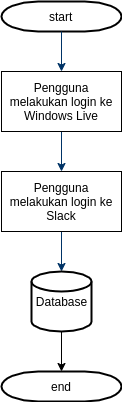
\includegraphics[width=3cm]{./Gambar/workflow.png}
      \centering
      \caption{Diagram alir sistem pada bagian perangkat lunak yang berinteraksi dengan \textit{user}.}
      \label{fig:workflow1}
    \end{figure}
    
    Diagram alir pada gambar \ref{fig:workflow1} menunjukkan aliran proses yang terjadi pada bagian perangkat lunak yang berinteraksi dengan pengguna, berikut penjelasan dari aliran proses tersebut:
    \begin{itemize}
        \item Proses pengguna melakukan \textit{login} ke \textit{Windows Live} adalah proses dimana perangkat lunak akan mendapatkan \textit{access token} dari \textit{Windows Live} dan data lainnya yang dibutuhkan untuk mendapatkan data dari \textit{event} yang tercatat di dalam \textit{Outlook Calendar}. 
        \item Proses pengguna melakukan \textit{login} ke \textit{Slack} adalah proses dimana perangkat lunak akan mendapatkan \textit{access token} dari \textit{Slack} untuk bisa mengganti status jika ada suatu \textit{event} yang berjalan. 
        \item Setelah kedua proses dijalankan, maka semua data yang dibutuhkan akan dimasukkan ke dalam \textit{database} agar bisa dijalankan juga dengan bagian dari perangkat lunak yang lain. 
    \end{itemize}
    
    \item \textbf{Bagian perangkat lunak yang dijalankan secara berkala}
    \begin{figure}[h]
      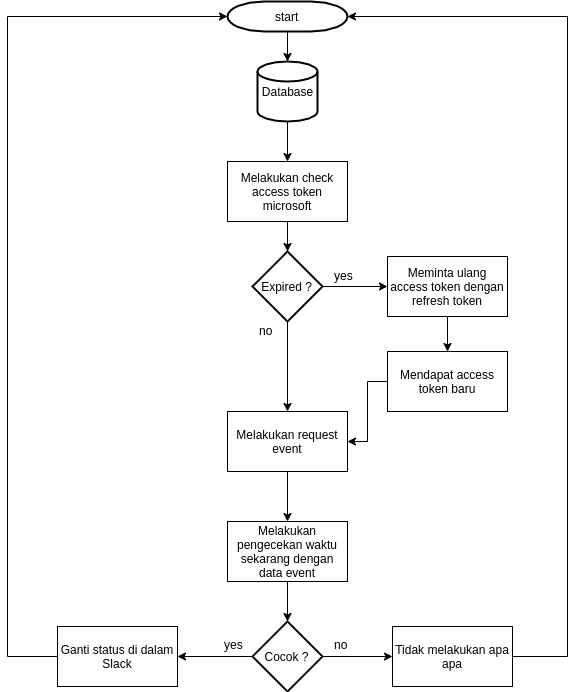
\includegraphics[width=10cm]{./Gambar/workflow2.png}
      \centering
      \caption{Diagram alir sistem pada bagian perangkat lunak yang dijalankan secara berkala.}
      \label{fig:workflow2}
    \end{figure}
    
    Diagram alir pada gambar \ref{fig:workflow2} menunjukkan aliran proses yang dilakukan oleh bagian perangkat lunak yang dijalankan secara berkala, berikut penjelasan dari aliran proses tersebut:
    \begin{itemize}
        \item Pertama-tama perangkat lunak akan mengambil data dari dalam basis data. 
        \item Lalu terdapat proses untuk melakukan pengecekan untuk \textit{access token} dari \textit{Microsoft} dikarenakan \textit{access token} ini memiliki waktu kadaluarsa. 
        \item Jika \textit{access token} sudah kadaluarsa, maka meminta ulang \textit{access token} dengan menggunakan \textit{refresh token}.
        \item Jika \textit{access token} belum \textit{expired}, maka dilanjutkan dengan meminta data mengenai \textit{event} yang ada di \textit{Outlook Calendar}. 
        \item Jika setelah melakukan permintaan ulang \textit{access token} dan sudah mendapatkan \textit{access token} yang baru, maka meminta data mengenai \textit{event} yang ada di \textit{Outlook Calendar}. 
        \item Lalu setelah mendapatkan data \textit{event}, maka melakukan pengecekan data \textit{event} dengan waktu sekarang. Jika waktu sekarang beririsan dengan \textit{event} yang sedang berjalan, maka perangkat lunak akan mengganti status yang ada pada \textit{Slack}. 
        \item Jika tidak ada yang beririsan, maka tidak akan melakukan apa-apa. 
        \item Proses ini akan berjalan kembali secara berkala sesuai dengan waktu yang sudah diatur di dalam \textit{Heroku Scheduler}. 
    \end{itemize}
\end{itemize}

Untuk bisa mendapatkan data \textit{event} yang disimpan pada aplikasi \textit{Outlook Calendar}, dibutuhkan analisis mengenai \textit{Microsoft Graph} seperti yang dijelaskan pada subbab \ref{sec:analisis_microsoft_graph_api}.

\subsection{Analisis \textit{Microsoft Graph API}}
\label{sec:analisis_microsoft_graph_api}

Pada analisis bagian ini, dilakukan analisis mengenai \textit{API} yang telah disediakan oleh \textit{Microsoft Graph API} yang akan digunakan untuk mengambil data acara / \textit{event} yang dibutuhkan oleh perangkat lunak yang akan dibangun. Akan ada beberapa langkah yang harus dijalankan untuk berhasil mencapai tujuan dari perangkat lunak ini. Analisis dari setiap langkah akan dijelaskan pada subbab \ref{analisis_authorization_code} sampai subbab \ref{analisis_menggunakan_refresh_token}.

\subsubsection{Analisis Mendapatkan \textit{Authorization Code}}
\label{analisis_authorization_code}
Untuk mendapatkan \textit{authorization code}, diperlukan untuk mendaftarkan aplikasi yang akan dibuat ke \textit{Microsoft App Registration Portal}\footnote{https://apps.dev.microsoft.com/}. Dari mendaftarkan aplikasi yang akan dibuat di portal registrasi tersebut akan menghasilkan \textit{Application ID}, \textit{Application Secret}, dan juga \textit{redirect URL} yang akan digunakan. Jika \textit{platform} yang dipilih adalah \textit{web}, maka \textit{redirect URL} harus ditentukan sendiri. Dalam meminta \textit{authorization code}, aplikasi yang dibuat harus mengirimkan \textit{get request} terlebih dahulu ke \textit{endpoint /authorize} yang membutuhkan \textit{parameter} seperti yang dijelaskan di tabel \ref{tab:parameter_authorization_code}. 

\begin{table}[H]
	\centering 
	\caption{Tabel \textit{parameter} \textit{Authorization Code}}
	\label{tab:parameter_authorization_code}
	\begin{tabular}{|p{3cm}|p{3cm}|p{9cm}|}
	\toprule
	\textbf{Parameter} & & \textbf{Deskripsi}\\ \hline 
	\textit{tenant} & wajib & Nilai \textit{tenant} berfungsi untuk mengontrol siapa yang dapat masuk ke dalam aplikasi. Bisa diisi dengan \textit{tenant ID} atau nama domain dari akun \textit{Microsoft}.\\ \hline 
	\textit{client\_id} & wajib & Nilai yang dipakai adalah nilai dari \textit{application ID} yang didapatkan saat mendaftarkan aplikasi di \textit{Microsoft App Registration Portal}.\\ \hline 
	\textit{response\_type} & wajib & Tipe balikan yang diterima dari \textit{request}. Bernilai 				\textit{code} yang berarti akan mengembalikan \textit{code}. \\ \hline 
	\textit{redirect\_uri} & direkomendasikan & \textit{Redirect uri} dari aplikasi yang didaftarkan dimana hasil dari \textit{request} yang didapat akan dikembalikan ke \textit{url} yang sudah didaftarkan. \\ \hline 
	\textit{scope} & wajib & Daftar izin dari \textit{Microsoft Graph} yang dipisahkan oleh cakupan yang diinginkan dan disetujui oleh pengguna. \\ \hline 
\textit{response\_mode} & direkomendasikan & Menentukan metode yang harus digunakan untuk mengirimkan \textit{token} yang dihasilkan kembali ke aplikasi. Dapat bernilai \textit{query} atau \textit{form\_post}. \\ \hline 
	\textit{state} & direkomendasikan & Nilai yang diisi saat mengirimkan \textit{request} dan akan dikembalikan juga saat menerima \textit{response}. Tujuan dari nilai ini adalah untuk mencegah pemalsuan permintaan lintas situs. Digunakan untuk menyandikan informasi sebelum \textit{request} untuk otentikasi. Biasanya nilai ini berisi nilai unik secara acak. \\ \bottomrule
\end{tabular}  
\end{table}

Pada \textit{parameter scope}, dapat diisi dengan nilai \textit{offline\_access} yang menjadikan aplikasi mendapatkan \textit{response} berupa \textit{refresh token} yang berguna untuk mendapatkan \textit{access token} yang baru saat yang lama sudah kadaluarsa. Contoh \textit{request} yang dikirimkan akan seperti yang terdapat pada contoh table \ref{tab:contoh_request_authorization_code}.

\begin{table}[H]
	\centering 
	\caption{Tabel contoh \textit{request} \textit{Authorization Code}}
	\label{tab:contoh_request_authorization_code}
	\begin{tabular}{|p{12cm}|}
	\toprule
	https://login.microsoftonline.com/\{tenant\}/oauth2/v2.0/authorize?\\
client\_id=6731de76-14a6-49ae-97bc-6eba6914391e\\
\&response\_type=code\\
\&redirect\_uri=http\%3A\%2F\%2Flocalhost\%2Fmyapp\%2F\\
\&response\_mode=query\\
\&scope=offline\_access\%20user.read\%20mail.read\\
\&state=12345\\
	\bottomrule
\end{tabular}  
\end{table}

Dari \textit{request} seperti contoh table \ref{tab:contoh_request_authorization_code}, akan menghasilkan contoh \textit{response} seperti yang terdapat pada table \ref{tab:contoh_response_authorization_code} dengan keterangan \textit{parameter} seperti yang terdapat pada table \ref{tab:parameter_response_authorization_code}. 

\begin{table}[H]
	\centering 
	\caption{Tabel contoh \textit{response} \textit{Authorization Code}}
	\label{tab:contoh_response_authorization_code}
	\begin{tabular}{|p{9cm}|}
	\toprule
	GET https://localhost/myapp/?\\
code=M0ab92efe-b6fd-df08-87dc-2c6500a7f84d\\
\&state=12345 \\
	\bottomrule
\end{tabular}  
\end{table}

\begin{table}[H]
	\centering 
	\caption{Tabel \textit{parameter} \textit{response} \textit{Authorization Code}}
	\label{tab:parameter_response_authorization_code}
	\begin{tabular}{|p{3cm}|p{9cm}|}
	\toprule
	\textbf{Parameter} & \textbf{Deskripsi}\\ \hline 
	\textit{code} & Nilai ini merupakan \textit{authorization\_code} yang telah di\textit{request} oleh aplikasi. \textit{Authorization\_code} ini digunakan untuk meminta \textit{access token}. \textit{Authorization code} memiliki waktu kadaluarsa yang singkat yaitu biasanya akan kadaluarsa setelah 10 menit. \\ \hline 
	\textit{state} & Jika saat melakukan \textit{request}, \textit{parameter} \textit{state} diisi, maka pada saat mengeluarkan \textit{response}, akan mengeluarkan nilai \textit{state} yang sama seperti yang sudah diisi saat melakukan \textit{request}. Aplikasi harus mengidentifikasi apakah nilai \textit{state} saat melakukan \textit{request} dengan nilai \textit{state} di \textit{response} sama atau tidak. \\ \bottomrule
\end{tabular}  
\end{table}

Hasil \textit{response} yang ditampilkan oleh table \ref{tab:contoh_response_authorization_code} muncul karena pada saat \textit{request} di table \ref{tab:contoh_request_authorization_code} terdapat \textit{parameter} \textit{response\_mode} yang diisi dengan nilai \textit{query} sehingga \textit{response} yang dikembalikan dalam bentuk \textit{query string} dari \textit{redirect url}. 

\subsubsection{Analisis Mendapatkan \textit{Access Token}}
\label{analisis_access_token}

Setelah mendapatkan \textit{authorization code}, langkah selanjutnya yang harus dijalankan sebelum bisa memanggil \textit{method API} yang dibutuhkan adalah dengan mendapatkan \textit{access token}. Yang diperlukan untuk bisa mendapatkan \textit{access token}, maka aplikasi yang dibuat membutuhkan \textit{authorization code} yang diterima di langkah sebelumnya dan mengirimkan \textit{post request} kepada \textit{endpoint /token}. 

Untuk mengirimkan \textit{post request}, diperlukan \textit{request body} yang memiliki elemen-elemen seperti yang terdapat di contoh table \ref{tab:contoh_request_access_token}. Adapun penjelasan dari setiap \textit{parameter} yang terdapat di dalam \textit{request body} dijelaskan pada table \ref{tab:parameter_request_access_token}. 

\begin{table}[H]
	\centering 
	\caption{Tabel contoh \textit{request} \textit{Access Token}}
	\label{tab:contoh_request_access_token}
	\begin{tabular}{|p{12cm}|}
	\toprule
	POST /common/oauth2/v2.0/token HTTP/1.1\\
Host: https://login.microsoftonline.com\\
Content-Type: application/x-www-form-urlencoded\\
\\
client\_id=6731de76-14a6-49ae-97bc-6eba6914391e\\
\&scope=user.read\%20mail.read\\
\&code=OAAABAAAAiL9Kn2Z27UubvWFPbm0gLWQ\\
JVzCTE9UkP3pSx1aXxUjq3n8b2JRLk4OxVXr...\\
\&redirect\_uri=http\%3A\%2F\%2Flocalhost\%2Fmyapp\%2F\\
\&grant\_type=authorization\_code\\
\&client\_secret=JqQX2PNo9bpM0uEihUPzyrh \\ 
	\bottomrule
	\end{tabular}  
\end{table}

\begin{table}[H]
	\centering 
	\caption{Tabel \textit{parameter} \textit{request} \textit{Access Token}}
	\label{tab:parameter_request_access_token}
	\begin{tabular}{|p{3cm}|p{3cm}|p{9cm}|}
	\toprule
	 \textbf{Parameter} & & \textbf{Deskripsi}\\ \hline 
	\textit{tenant} & wajib & Nilai \textit{tenant} berfungsi untuk mengontrol siapa yang dapat masuk ke dalam aplikasi. Bisa diisi dengan \textit{tenant ID} atau nama \textit{domain} dari akun \textit{Microsoft}.\\ \hline 
	\textit{client\_id} & wajib & Nilai yang dipakai adalah nilai dari \textit{application ID} yang didapatkan saat mendaftarkan aplikasi di \textit{Microsoft App Registration Portal}.\\ \hline 
	\textit{grant\_type} & wajib & Harus diisi dengan nilai \textit{authorization\_code} untuk alur \textit{authorization code}. \\ \hline
	\textit{scope} & wajib & Daftar izin dari \textit{Microsoft Graph} yang dipisahkan oleh cakupan yang diinginkan dan disetujui oleh pengguna. Dalam langkah ini, nilai dari \textit{scope} pada langkah sebelumnya harus sama dengan langkah ini.  \\ \hline 
	\textit{code} & wajib & \textit{Authorization code} yang didapat dari langkah sebelumnya. \\ \hline  
	\textit{redirect\_uri} & wajib & \textit{Redirect uri} yang sama yang dipakai untuk mendapatkan \textit{authorization code}. \\ \hline 
	\textit{client\_secret} & wajib untuk \textit{web apps} & \textit{Application secret} yang dibuat saat mendaftarkan aplikasi di portal registrasi untuk aplikasi yang didaftarkan.\\
	\bottomrule
	\end{tabular}  
\end{table}

Dari contoh \textit{request} yang dilakukan pada table\ref{tab:contoh_request_access_token}, maka akan dihasilkan contoh \textit{token} seperti pada table \ref{tab:contoh_response_access_token} yang memiliki keterangan dari hasil yang dikembalikan pada table\ref{tab:parameter_response_access_token}. 

\begin{table}[H]
	\centering 
	\caption{Tabel contoh \textit{response} \textit{Access Token}}
	\label{tab:contoh_response_access_token}
	\begin{tabular}{|p{9cm}|}
	\toprule
	\{\\
    "token\_type": "Bearer",\\
    "scope": "user.read\%20Fmail.read",\\
    "expires\_in": 3600,\\
    "access\_token": "eyJ0eXAiOiJKV1QiLCJhbG\\
    ciOiJSUzI1NiIsIng1dCI6Ik5HVEZ2ZEstZnl0aEV1Q...",\\
    "refresh\_token": "AwABAAAAvPM1KaPlrEqdF\\
    SBzjqfTGAMxZGUTdM0t4B4..."\\
	\}\\ 
	\bottomrule
	\end{tabular}  
\end{table}

\begin{table}[H]
	\centering 
	\caption{Tabel \textit{parameter} \textit{response} \textit{Access Token}}
	\label{tab:parameter_response_access_token}
	\begin{tabular}{|p{3cm}|p{9cm}|}
	\toprule
	 \textbf{Parameter} & \textbf{Deskripsi}\\ \hline 
	\textit{token\_type} & Menunjukkan nilai dari \textit{token}. Satu-satunya jenis \textit{token} yang didukung oleh \textit{Azure AD} adalah \textit{Bearer}.\\ \hline 
	\textit{scope} & Nilai \textit{scope} yang \textit{valid} untuk \textit{access\_token} yang diberikan.  \\ \hline 
	\textit{expires\_in} & Lamanya \textit{access token} akan berlaku(dalam detik). \\ \hline  
	\textit{access\_token} & \textit{Access token} yang diminta. Dengan memakai ini, maka aplikasi bisa memanggil \textit{Microsoft Graph}. \\ \hline 
	\textit{refresh\_token} & \textit{Refresh token} ini berguna untuk meminta kembali \textit{access token} setelah \textit{access token} itu berakhir. \textit{Refresh token} memiliki umur yang panjang dan dapat digunakan untuk mempertahankan akses ke \textit{source}. \\
	\bottomrule
	\end{tabular}  
\end{table}

\subsubsection{Analisis Menggunakan \textit{Access Token} untuk memanggil \textit{Microsoft Graph}}
\label{analisis_menggunakan_access_token}
Setelah mendapatkan \textit{access token}, panggilan ke \textit{Microsoft Graph} pun bisa dilakukan dengan syarat menyertakan \textit{access token} di \textit{authorization header} di setiap \textit{request} yang dikirim. Pada table\ref{tab:contoh_request_call_microsoft_graph} menunjukkan contoh \textit{request} untuk mendapatkan \textit{profile} dari pengguna yang masuk. 

\begin{table}[H]
	\centering 
	\caption{Tabel contoh \textit{request} \textit{call Microsoft Graph}}
	\label{tab:contoh_request_call_microsoft_graph}
	\begin{tabular}{|p{9cm}|}
	\toprule
	GET https://graph.microsoft.com/v1.0/me \\
Authorization: Bearer eyJ0eXAiO ... 0X2tnSQLEANnSPHY0gKcgw\\
Host: graph.microsoft.com \\
	\bottomrule
	\end{tabular}  
\end{table}

Jika \textit{request} yang dikirimkan berhasil, maka akan mendapatkan \textit{response} yang akan terlihat mirip dengan contoh seperti pada table \ref{tab:contoh_response_call_microsoft_graph}

\begin{table}[H]
	\centering 
	\caption{Tabel contoh \textit{response} \textit{call Microsoft Graph}}
	\label{tab:contoh_response_call_microsoft_graph}
	\begin{tabular}{|p{12cm}|}
	\toprule
	HTTP/1.1 200 OK\\
Content-Type: application/json;\\
odata.metadata=minimal;\\
odata.streaming=true;\\
IEEE754Compatible=false;\\
charset=utf-8\\
\\
request-id: f45d08c0-6901-473a-90f5-7867287de97f\\
client-request-id: f45d08c0-6901-473a-90f5-7867287de97f\\
OData-Version: 4.0\\
Duration: 727.0022\\
Date: Thu, 20 Apr 2017 05:21:18 GMT\\
Content-Length: 407\\
\\
\{\\
    "@odata.context":"https://graph.microsoft.com/v1.0/\\
    $metadata\#users/$entity",\\
    "id":"12345678-73a6-4952-a53a-e9916737ff7f",\\
    "businessPhones":[\\
        "+1 555555555"\\
    ],\\
    "displayName":"Chris Green",\\
    "givenName":"Chris",\\
    "jobTitle":"Software Engineer",\\
    "mail":null,\\
    "mobilePhone":"+1 5555555555",\\
    "officeLocation":"Seattle Office",\\
    "preferredLanguage":null,\\
    "surname":"Green",\\
    "userPrincipalName":"ChrisG@contoso.onmicrosoft.com"\\
\}\\
	\bottomrule
	\end{tabular}  
\end{table}

\subsubsection{Analisis Menggunakan \textit{Refresh Token} untuk Mendapatkan \textit{Access Token} Baru}
\label{analisis_menggunakan_refresh_token}
\textit{Access token} memiliki waktu yang singkat dan ketika sudah kadaluarsa, maka aplikasi yang akan dibuat harus meminta kembali \textit{access token} supaya bisa terus mengakses data yang ada di dalam \textit{Microsoft Graph}. Cara mendapatkan \textit{access token} yang baru dengan menggunakan \textit{refresh token} adalah dengan cara mengirimkan \textit{post request} sekali lagi kepada \textit{endpoint /token} dengan menggunakan \textit{refresh token} sebagai \textit{parameter} yang dikirimkan dan juga \textit{grant type} yang berisikan \textit{refresh token} dalam \textit{body} dari \textit{request} yang dilakukan seperti contoh pada table \ref{tab:contoh_request_refresh_token} dengan keterangan \textit{parameter} seperti yang dijelaskan pada table \ref{tab:parameter_request_refresh_token}. 

\begin{table}[H]
	\centering 
	\caption{Tabel contoh \textit{request} menggunakan \textit{Refresh Token}}
	\label{tab:contoh_request_refresh_token}
	\begin{tabular}{|p{12cm}|}
	\toprule
	POST /common/oauth2/v2.0/token HTTP/1.1\\
Host: https://login.microsoftonline.com\\
Content-Type: application/x-www-form-urlencoded\\
\\
client\_id=6731de76-14a6-49ae-97bc-6eba6914391e\\
\&scope=user.read\%20mail.read\\
\&refresh\_token=OAAABAAAAiL9Kn2Z27UubvWFPbm0gLWQJVzCTE\\
9UkP3pSx1aXxUjq...\\
\&redirect\_uri=http\%3A\%2F\%2Flocalhost\%2Fmyapp\%2F\\
\&grant\_type=refresh\_token\\
\&client\_secret=JqQX2PNo9bpM0uEihUPzyrh\\
	\bottomrule
	\end{tabular}  
\end{table}

\begin{table}[H]
	\centering 
	\caption{Tabel \textit{parameter} \textit{request} \textit{Refresh Token}}
	\label{tab:parameter_request_refresh_token}
	\begin{tabular}{|p{3cm}|p{3cm}|p{9cm}|}
	\toprule
	 \textbf{Parameter} & & \textbf{Deskripsi}\\ \hline 
	\textit{client\_id} & wajib & Nilai yang dipakai adalah nilai dari \textit{application ID} yang didapatkan saat mendaftarkan aplikasi di \textit{Microsoft App Registration Portal}.\\ \hline 
	\textit{grant\_type} & wajib & Harus diisi dengan nilai \textit{refresh\_token}. \\ \hline
	\textit{scope} & wajib & Daftar izin dari \textit{Microsoft Graph} yang dipisahkan oleh cakupan yang diinginkan dan disetujui oleh pengguna. Dalam langkah ini, nilai dari \textit{scope} pada langkah meminta \textit{authorization\_code} harus sama dengan langkah ini.  \\ \hline 
	\textit{refresh\_token} & wajib & \textit{Refresh token} yang didapat saat melakukan \textit{request token} yang pertama kali. \\ \hline  
	\textit{redirect\_uri} & wajib & \textit{Redirect uri} yang sama yang dipakai untuk mendapatkan \textit{authorization code}. \\ \hline 
	\textit{client\_secret} & wajib untuk \textit{web apps} & \textit{Application secret} yang dibuat saat mendaftarkan aplikasi di portal registrasi untuk aplikasi yang didaftarkan.\\
	\bottomrule
	\end{tabular}  
\end{table}

Jika \textit{request} ini berhasil, maka akan mengembalikan \textit{response} seperti pada table \ref{tab:contoh_response_refresh_token} yang memiliki keterangan \textit{parameter} yang dikembalikannya seperti pada table \ref{tab:parameter_response_refresh_token}. 
\\
\begin{table}[H]
	\centering 
	\caption{Tabel contoh \textit{response} menggunakan \textit{Refresh Token}}
	\label{tab:contoh_response_refresh_token}
	\begin{tabular}{|p{12cm}|}
	\toprule
	\{\\
    "access\_token": "eyJ0eXAiOiJKV1QiLCJhbGciOiJSUzI1NiI\\
    sIng1dCI6Ik5HVEZ2ZEstZnl0aEV1Q...",\\
    "token\_type": "Bearer",\\
    "expires\_in": 3599,\\
    "scope": "user.read\%20mail.read",\\
    "refresh\_token": "AwABAAAAvPM1KaPlrEqdFSBzjq\\
    fTGAMxZGUTdM0t4B4...",\\
\}\\
	\bottomrule
	\end{tabular}  
\end{table}

\begin{table}[H]
	\centering 
	\caption{Tabel \textit{parameter} \textit{response} \textit{Refresh Token}}
	\label{tab:parameter_response_refresh_token}
	\begin{tabular}{|p{3cm}|p{9cm}|}
	\toprule
	 \textbf{Parameter} & \textbf{Deskripsi}\\ \hline 
	 \textit{access\_token} & \textit{Access token} yang diminta. Dengan memakai ini, maka aplikasi bisa memanggil \textit{Microsoft Graph}. \\ \hline 
	\textit{token\_type} & Menunjukkan nilai dari \textit{token}. Satu-satunya jenis \textit{token} yang didukung oleh \textit{Azure AD} adalah \textit{Bearer}.\\ \hline 
	\textit{expires\_in} & Lamanya \textit{access token} akan berlaku(dalam detik). \\ \hline 
	\textit{scope} & Nilai \textit{scope} yang valid untuk \textit{access\_token} yang diberikan.  \\ \hline  
	\textit{refresh\_token} & \textit{Refresh token} ini berguna untuk meminta kembali \textit{access token} setelah \textit{access token} itu berakhir. \textit{Refresh token} memiliki umur yang panjang dan dapat digunakan untuk mempertahankan akses ke \textit{source}. \\
	\bottomrule
	\end{tabular}  
\end{table}

\subsubsection{Analisis Mendapatkan Data \textit{Events}}
\label{sec:analisis_mendapatkan_data_events}
Data \textit{event} di dalam \textit{Microsoft Graph} tersimpan di dalam objek \textit{event} yang memiliki relasi dengan objek \textit{user} dari pengguna. Untuk dapat mengakses \textit{event} yang memiliki relasi dengan \textit{user}, aplikasi yang dibuat harus menjalankan \textit{method} yang dimiliki objek \textit{user} yaitu \textit{method list events}. Cara menggunakan \textit{method} ini adalah dengan mengirimkan \textit{get request} kepada \textit{endpoint /me/events}. \textit{List events} sendiri adalah method yang berfungsi untuk mengembalikan objek-objek \textit{event} yang berkaitan dengan objek \textit{user} pengguna. Untuk setiap operasi \textit{get} yang mengembalikan objek \textit{event} di \textit{Microsoft Graph}, ada sebuah \textit{parameter header} ``\textit{Prefer:outlook.timezone}'' yang berfungsi untuk menentukan \textit{time zone} untuk mulainya dan berakhirnya \textit{event}. Sebagai contoh, dapat dilihat pada table \ref{tab:contoh_header_time_zone}. 

\begin{table}[H]
	\centering 
	\caption{Tabel contoh \textit{header time zone}}
	\label{tab:contoh_header_time_zone}
	\begin{tabular}{|p{9cm}|}
	\toprule
	 Prefer: outlook.timezone="Eastern Standard Time" \\
	\bottomrule
	\end{tabular}  
\end{table}

Pada table \ref{tab:contoh_header_time_zone}, \textit{outlook timezone} diatur menjadi \textit{Eastern Standard Time} yang nantinya semua \textit{event} yang dipanggil dengan \textit{header} seperti itu akan mengembalikan \textit{starttime} dan \textit{endtime} dari \textit{event} akan disesuaikan dengan zona waktu \textit{Eastern Standard Time}. 

Untuk bisa mengakses \textit{method} ini, maka diperlukan \textit{format header} dari \textit{request} seperti yang akan dijelaskan pada table \ref{tab:parameter_header_time_zone}. 

\begin{table}[H]
	\centering 
	\caption{Tabel \textit{parameter} \textit{header time zone}}
	\label{tab:parameter_header_time_zone}
	\begin{tabular}{|p{3cm}|p{3cm}|p{9cm}|}
	\toprule
	 \textbf{Nama} & \textbf{\textit{Type}} & \textbf{Deskripsi}\\ \hline
	 \textit{Authorization} & \textit{String} & \textit{Bearer {token}}. Bersifat wajib diisi. \\ \hline
	 \textit{Prefer:}& & \\
	 \textit{outlook.timezone} & \textit{String} & Digunakan untuk menentukan zona waktu yang akan dipakai untuk data yang akan dikembalikan. Bersifat optional. \\ \hline
	 \textit{Prefer:}& & \\
	 \textit{outlook.body-content-type} & \textit{String} & Merupakan nilai yang mengatur properti dari \textit{response body} yang akan dikembalikan. Nilai bisa berupa ``\textit{text}'' atau ``\textit{html}''. Nilai \textit{default} dari \textit{parameter} ini adalah \textit{html}. Bersifat optional. \\ \hline
	\bottomrule
	\end{tabular}  
\end{table}

\textit{Request} ini mengembalikan \textit{response} berupa \textit{json} objek dari \textit{event resource type}. \textit{Request} ini juga bisa menerima \textit{parameter} \$select yang berbentuk \textit{string query} sebagai \textit{filter} mengenai \textit{field} yang mau diambil dari objek \textit{event}. Dapat dilihat fungsi dari \textit{parameter string query} \$select seperti pada contoh table \ref{tab:contoh_request_event} dan contoh \textit{response}nya pada table \ref{tab:contoh_response_event}. 

\begin{table}[H]
	\centering 
	\caption{Tabel contoh \textit{request event}}
	\label{tab:contoh_request_event}
	\begin{tabular}{|p{12cm}|}
	\toprule
	GET https://graph.microsoft.com/v1.0/me/events?\\
	\$select=subject,bodyPreview,organizer,start,end,location\\
	Prefer: outlook.timezone="Pacific Standard Time"\\
	\bottomrule
	\end{tabular}  
\end{table}

\begin{table}[H]
	\centering 
	\caption{Tabel contoh \textit{response event}}
	\label{tab:contoh_response_event}
	\begin{tabular}{|p{15cm}|}
	\toprule
	\begin{lstlisting}
{
    "@odata.context":"https://graph.microsoft.com/v1.0/$metadata
    #users('cd209b0b-3f83-4c35-82d2-d88a61820480')/events(subject
    ,bodyPreview,organizer,start,end,location)",
    "value":[
        {
            "@odata.etag":"W/\"ZlnW4RIAV06KYYwlrfNZvQAAKGWwbw==\"",
            "id":"AAMkAGIAAAoZDOFAAA=",
            "subject":"Orientation ",
            "bodyPreview":"Dana, this is the time you selected for 
            our orientation. Please bring the notes I sent you.",
            "start":{
                "dateTime":"2017-04-21T10:00:00.0000000",
                "timeZone":"Pacific Standard Time"
            },"end":{
                "dateTime":"2017-04-21T12:00:00.0000000",
                "timeZone":"Pacific Standard Time"
            },"location": {
                "displayName": "Assembly Hall",
                "locationType": "default"
            },"locations": [{
                    "displayName": "Assembly Hall",
                    "locationType": "default"
            }],                
            "organizer":{
                "emailAddress":{
                    "name":"Samantha Booth",
                    "address":"samanthab@a830edad905084922E170
                    20313.onmicrosoft.com"
                }
            }
        }
    ]
}
\end{lstlisting}\\
	\bottomrule
	\end{tabular}  
\end{table}

Setelah melakukan analisis kepada aplikasi \textit{Outlook Calendar} melalui \textit{Microsoft Graph API} yang dipakai, maka sekarang akan dijelaskan analisis mengenai bagian dari perangkat lunak yang berinteraksi dengan aplikasi \textit{Slack} pada subbab \ref{sec:analisis_slack}.

\subsection{Analisis \textit{Slack}}
\label{sec:analisis_slack}
Pada bagian ini akan dijelaskan mengenai analisis pada aplikasi \textit{Slack}. Yang akan dibahas antara lain adalah analisis mengenai Status yang terdapat pada aplikasi \textit{Slack} yang akan dijelaskan pada bagian \ref{sec:analisis_status}. Lalu akan dilanjutkan dengan analisis cara menggunakan \textit{API} yang sudah disediakan oleh aplikasi \textit{Slack} untuk perangkat lunak bisa mengakses kepada aplikasi \textit{Slack} yang akan dibahas pada bagian \ref{sec:analisis_slack_api}

\subsubsection{Analisis Status pada \textit{Slack}}
\label{sec:analisis_status}
Status pada aplikasi \textit{Slack} adalah fitur yang menggambarkan kondisi dari pengguna saat itu dan fitur itu tergabung dalam profil dari pengguna. Status di dalam aplikasi \textit{Slack} sendiri terdiri dari 2 bagian yaitu sebuah simbol yang menggambarkan kondisi dari status, serta sebuah \textit{text} yang memperjelas keadaan dari status yang dialami oleh pengguna. Umumnya, \textit{Slack} menyediakan sebuah \textit{field} untuk pengguna bisa mengisi statusnya sesuai dengan keadaan yang dialami oleh pengguna. Ada juga beberapa status yang sudah disediakan oleh aplikasi \textit{Slack}. 

Perangkat lunak ini akan mengubah status pengguna dengan menggunakan simbol \textit{no entry sign}, dan juga \textit{text} yang bertuliskan ``\textit{In a meeting}''. Hal itu dipilih karena beberapa alasan yaitu:
\begin{itemize}
    \item Tujuan dari disusunnya perangkat lunak ini adalah untuk meminimalisir pengguna mendapatkan gangguan berupa \textit{chat} dari pengguna lain saat ada \textit{event} yang berlangsung, sehingga cocok untuk memasang status yang menggambarkan bahwa pengguna saat ini sedang tidak bisa diganggu. 
    \item Jika menggunakan pemeriksaan kata-kata di dalam \textit{subject} dari \textit{event}, maka akan muncul beberapa ambigu seperti contohnya jika di dalam \textit{subject} terdapat kata ``liburan'', maka perangkat lunak akan mengganti status menjadi ``\textit{On vacation}'', dan jika ada kata ``Rapat'', maka status akan menjadi ``\textit{In a meeting}'', lalu jika \textit{subject} dari \textit{event} adalah ``Rapat untuk membahas liburan bersama kerabat kerja'', status akan berganti menjadi ``\textit{On vacation}'' karena di dalam \textit{subject} mengandung kata liburan, tetapi seharusnya status berubah menjadi ``\textit{In a meeting}'' karena mengandung kata-kata utama yaitu ``Rapat''. 
    \item Jika menggunakan \textit{tag} khusus di dalam \textit{subject event}, maka akan menimbulkan banyak kondisi yang harus di \textit{handle} seperti contohnya bila dalam sebuah \textit{subject event} terdapat \textit{tag} ``[Rapat]'', maka status berganti menjadi ``\textit{In a meeting}'', dan jika ``[Liburan]'', maka status berganti menjadi ``\textit{On vacation}''. Jika ada \textit{subject} yang tidak menggunakan \textit{tag}, maka tidak tahu akan masuk ke dalam kategori status yang mana, atau bisa saja statusnya menjadi kosong padahal pengguna lupa untuk mengisi \textit{subject} pada \textit{event} dengan menggunakan \textit{tag}. Lalu jika ada kasus \textit{tag} yang belum dikenali oleh perangkat lunak, maka status yang dipasang juga menjadi kosong. 
\end{itemize}

Alasan-alasan diatas yang memperkuat pemilihan status yang akan dipasang oleh perangkat lunak ini secara otomatis yaitu dengan simbol ``\textit{no-entry}'', dan \textit{text} ``\textit{In a meeting}''. 

\subsubsection{Analisis \textit{Slack API}}
\label{sec:analisis_slack_api}
Pada bagian ini akan dibahas mengenai cara penggunaan \textit{Slack API}. Untuk dapat memakai dan mengakses \textit{method-method} yang disediakan oleh \textit{Slack}, dibutuhkan mendaftarkan aplikasi yang akan dibuat untuk bisa memperoleh \textit{Client ID} yang nantinya dibutuhkan untuk bisa mendapatkan \textit{authorization code} serta \textit{access token}. Sama seperti di \textit{Microsoft Graph API}, di dalam \textit{Slack API access token} dibutuhkan sebagai otorisasi untuk bisa mengakses \textit{method-method} yang disediakan oleh \textit{Slack}. Jika tidak memiliki \textit{access token}, maka seluruh \textit{method} yang dicoba di\textit{request} tidak akan mengembalikkan hasil dan dianggap sebagai \textit{request} yang tidak \textit{valid}. 

Pada sesi ini akan dibutuhkan \textit{method} dari \textit{Slack API} yang bisa mengubah status yang terdapat pada bagian \textit{user.profile}. Dari informasi yang disediakan oleh \textit{Slack} secara \textit{online}, bahwa status tergabung dalam \textit{user.profile}, maka untuk memenuhi dari kebutuhan di sisi ini dicoba menggunakan \textit{method-method} yang bisa untuk mengakses kepada objek \textit{user.profile}. Karena di sisi ini akan mengubah nilai dari status, asumsi sementara dari \textit{method} yang bisa dipakai dari sisi ini adalah \textit{method users.profile.set} yang akan berguna untuk mengubah isi dari profil pengguna yang di dalamnya terdapat status. 

Setelah analisis mengenai \textit{Slack}, maka pada bagian \ref{sec:analisis_heroku} akan membahas mengenai \textit{Heroku}. 

\subsection{Analisis \textit{Heroku}}
\label{sec:analisis_heroku}
Pada bagian ini akan membahas mengenai \textit{Heroku}. \textit{Heroku} adalah \textit{platform} yang dipakai untuk menyimpan perangkat lunak yang dibangun. Layaknya sebuah \textit{server}, \textit{heroku} akan menyimpan perangkat lunak dan jika berbasis \textit{web}, maka \textit{heroku} akan memberikan \textit{subdomain} agar perangkat lunak yang disimpan bisa diakses dan dijalankan secara langsung dengan mengakses \textit{subdomain} yang diberikan. Untuk \textit{heroku} yang berpaket gratis, maka akan ada keterbatasan seperti, perangkat lunak akan masuk ke dalam keadaan \textit{sleep} setiap 30 menit sekali jika tidak ada akses selama 30 menit kepada perangkat lunak dan perangkat lunak akan kembali aktif setelah ada akses kembali ke perangkat lunak dengan adanya sedikit keterlambatan saat memasuki keadaan aktif kembali. Lalu batasan lainnya adalah adanya batasan \textit{dyno hours} yang didapatkan yaitu sebesar 1000 jam jika akun sudah terverifikasi. Pada \textit{heroku} juga terdapat banyak \textit{add-ons} yang membantu fungsi dari perangkat lunak yang dibangun agar berjalan dengan baik, seperti basis data dan juga \textit{scheduler} yang berfungsi untuk menjalankan bagian dari perangkat lunak secara berkala. Untuk analisis dari \textit{add-ons}, akan dibahas pada bagian \ref{sec:analisis_postgres} dan juga \ref{sec:analisis_cron}. 

\subsubsection{Analisis \textit{Postgres}}
\label{sec:analisis_postgres}
\textit{Postgres} adalah basis data yang disediakan sebagai \textit{add-ons} pada \textit{heroku}. Untuk bisa mengaksesnya, bisa menggunakan \textit{Command Line Interface} (\textit{CLI}), atau juga bisa dibantu dengan menggunakan \textit{pgAdmin4}. Dengan menggunakan \textit{pgAdmin4} yang terkoneksi dengan \textit{url} yang diberikan oleh \textit{heroku} untuk mengakses \textit{postgres}, maka basis data yang tersimpan di \textit{heroku} bisa secara langsung terakses melalui \textit{pgAdmin4}. Cara melakukan koneksi dari \textit{pgAdmin4} ke \textit{url} yang sudah disediakan oleh \textit{heroku} adalah dengan membuat koneksi yang diisi dengan kredensial yang diberikan oleh \textit{heroku} pada halaman seperti pada gambar \ref{fig:postgres}. 

\begin{figure}[h]
  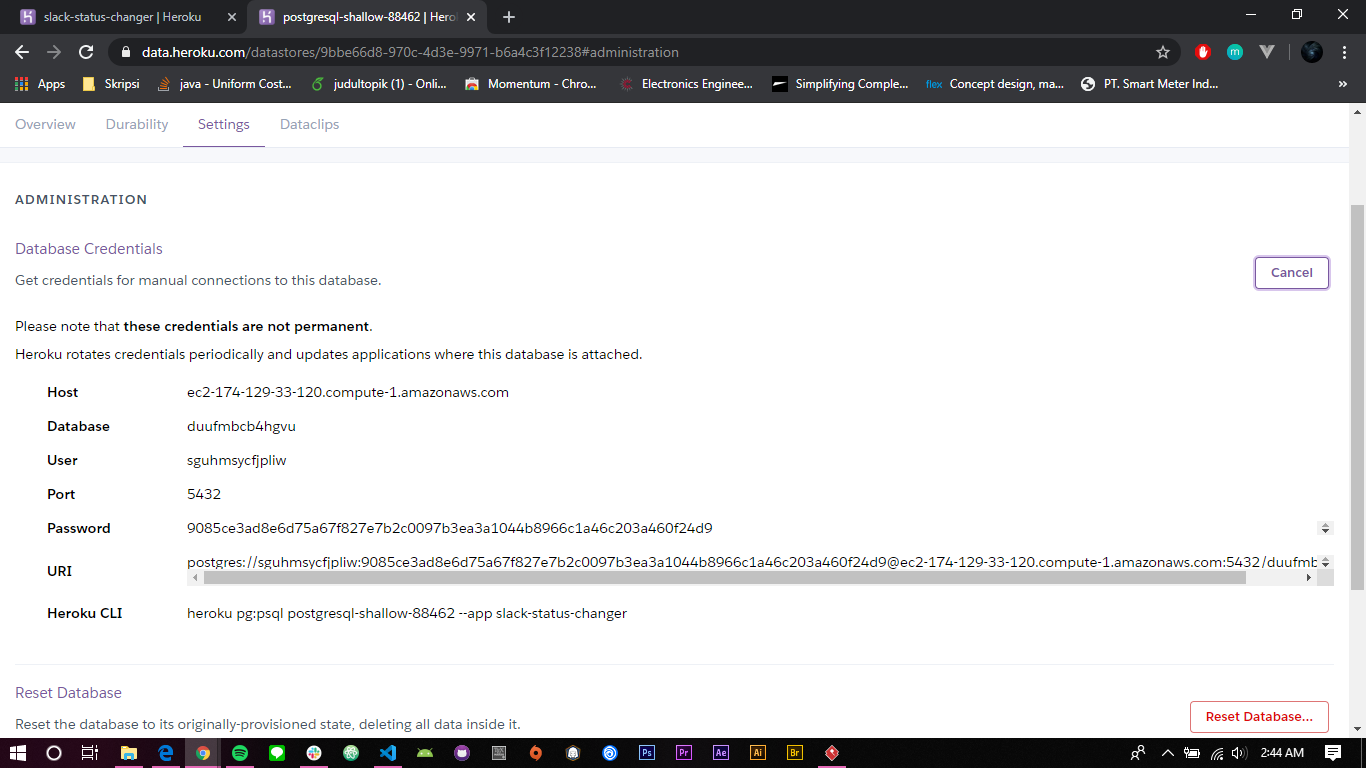
\includegraphics[width=15cm]{./Gambar/postgres.png}
  \centering
  \caption{Data kredensial yang diberikan oleh \textit{heroku postgres}.}
  \label{fig:postgres}
\end{figure}

Setelah memasukkan data kredensial yang diberikan oleh \textit{heroku postgres} ke \textit{pgAdmin4} dengan benar, maka koneksi akan tersambung ke basis data yang dibuat di \textit{postgres}. Selanjutnya dari \textit{pgAdmin4}, kegiatan \textit{create, update, insert, dan delete} terhadap basis data bisa dilakukan dengan cara penggunaan \textit{SQL syntax} seperti biasanya. Pada \textit{postgres}, akan dibutuhkan sebuah tabel yang akan menampung data-data yaitu:
\begin{itemize}
    \item \textbf{\textit{Microsoft Access Token}}\\
    \textit{Microsoft access token} adalah \textit{access token} dari pengguna yang didapat dari aplikasi \textit{Outlook Calendar}. 
    \item \textbf{\textit{Slack Access Token}}\\
    \textit{Slack access token} adalah \textit{access token} dari pengguna yang didapat dari aplikasi \textit{Slack}. 
    \item \textbf{\textit{Username}}\\
    \textit{Username} ini adalah penanda dari setiap pengguna yang akan bersifat identik. 
    \item \textbf{\textit{Microsoft Refresh Token}}\\
    \textit{Microsoft refresh token} adalah \textit{refresh token} dari \textit{Outlook Calendar} yang berfungsi untuk meminta ulang \textit{access token} jika \textit{access token} sudah kadaluarsa.
    \item \textbf{\textit{Microsoft Access Token Expiration Time}}\\
    \textit{Microsoft access token expiration time} ini adalah data yang mencatat masa kadaluarsa dari \textit{access token Outlook Calendar}. 
\end{itemize}

Setelah menganalisis \textit{postgres} yang digunakan sebagai basis data untuk perangkat lunak ini, maka akan dilanjutkan melakukan analisis \textit{heroku scheduler} yang berperan sebagai pengeksekusi perangkat lunak secara berkala pada bagian \ref{sec:analisis_cron}

\subsubsection{Analisis \textit{Heroku Scheduler}}
\label{sec:analisis_cron}
Untuk menjalankan aplikasi yang akan dibuat untuk mengambil data dari \textit{Microsoft Graph} yang berhubungan dengan pengambilan data \textit{event}, maka diperlukan aplikasi yang bisa mengambil data dengan mengirimkan \textit{request} kepada \textit{Microsoft Graph}, tetapi pengambilan data dibutuhkan secara berkala untuk memeriksa secara berkala data yang sudah dimasukkan ke dalam \textit{Microsoft Graph}. \textit{Heroku Scheduler} merupakan \textit{add-ons} dari \textit{Heroku} yang dapat menjalankan perintah secara berkala sesuai dengan yang sudah diatur sejak awal. Untuk menambahan \textit{job} pada \textit{Heroku Scheduler}, dapat diakses melalui \textit{command line} dengan perintah seperti:

\begin{lstlisting}
$ heroku addons:open scheduler
\end{lstlisting}

Setelah halaman baru pada \textit{browser} muncul, pilih tombol untuk menambahkan \textit{job} di \textit{scheduler} dengan menekan tombol ``\textit{Add Job}''. Pada \textit{Heroku Scheduler} tersedia interval untuk menjalankan sebuah \textit{job} yaitu setiap 10 menit sekali, atau setiap jam pada menit ke, atau setiap hari pada jam ke. Interval paling pendek untuk setiap kali iterasi yang disediakan oleh \textit{heroku scheduler} adalah setiap 10 menit sekali. 

Untuk memperkecil perangkat lunak melewatkan \textit{event} yang tercatat di \textit{Outlook Calendar} dan memaksimalkan iterasi dari \textit{heroku scheduler}, maka bagian dari perangkat lunak yang melakukan sinkronisasi akan dijalankan setiap 10 menit sekali. 


\subsection{Analisis \textit{Data Flow Diagram}}

Pada bagian ini akan menjelaskan mengenai aliran data yang terjadi pada proses di dalam perangkat lunak ini.

\begin{figure}[h]
  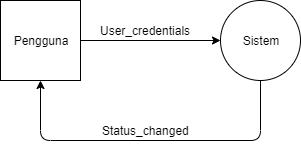
\includegraphics[width=15cm]{./Gambar/DFDlvl0.png}
  \centering
  \caption{\textit{Data Flow Diagram level} 0.}
  \label{fig:dfdlvl0}
\end{figure}

Diagram alir data pada gambar \ref{fig:dfdlvl0} menunjukkan aliran data pada sistem yang menerima input dari pengguna berupa user\_credentials yang berisi data dari pengguna untuk melakukan login seperti username dan password yang dimiliki oleh pengguna. Lalu di dalam sistem, ada berbagai proses yang dijabarkan pada gambar \ref{fig:dfd}. 

\begin{figure}[h]
  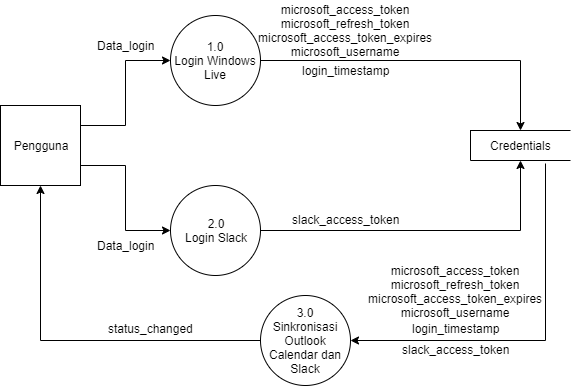
\includegraphics[width=15cm]{./Gambar/DFDlvl1.png}
  \centering
  \caption{\textit{Data Flow Diagram}.}
  \label{fig:dfd}
\end{figure}

Diagram alir data pada gambar \ref{fig:dfd} menunjukkan aliran data pada sistem, berikut penjelasan dari setiap proses aliran data tersebut:
\begin{itemize}
    \item \textbf{Proses melakukan \textit{login} ke \textit{Windows Live}}\\
    Input : ID dan Password akun Windows Live.\\
    Output : microsoft\_access\_token, microsoft\_access\_token\_expires, microsoft\_refresh\_token, microsoft\_username, login\_timestamp\\
    Proses ini merupakan proses meminta access token dan segala data yang diperlukan untuk mendapatkan data event dari Outlook Calendar. Proses ini menghasilkan data microsoft\_access\_token, microsoft\_access\_token\_expires, microsoft\_refresh\_token, microsoft\_username, dan login\_timestamp yang disimpan ke tabel Credentials sebagai data store. 
    \item \textbf{Proses melakukan \textit{login} ke \textit{Slack}}\\
    Input : \textit{ID} dan \textit{Password} beserta \textit{workspace} di \textit{Slack}.\\
    Output : slack\_access\_token\\
    Proses ini merupakan proses meminta access token kepada aplikasi Slack agar perangkat lunak bisa mengubah status di dalam aplikasi Slack. Proses ini menghasilkan data slack\_access\_token yang disimpan ke tabel Credentials sebagai data store. 
    \item \textbf{Proses melakukan sinkronisasi antara Outlook Calendar dan Slack}\\
    Input : microsoft\_access\_token, microsoft\_access\_token\_expires, microsoft\_refresh\_token, microsoft\_username, login\_timestamp, dan slack\_access\_token\\
    Output : Status di slack yang terubah jika memenuhi kondisi. 
    Proses ini merupakan proses sinkronisasi aplikasi Outlook Calendar dan juga Slack dengan cara mengambil data event yang terdapat di Outlook Calendar menggunakan token yang didapat dari Windows Live dan juga menggunakan token yang didapat dari Slack untuk dapat mengubah status dalam Slack jika waktu event dan waktu sekarang beririsan. 
\end{itemize}

\section{Analisis Kasus}
Pada perangkat lunak ini, akan ada kasus diluar pola dari kasus normalnya yaitu adanya kasus dimana akan ada jadwal yang bertabrakan contohnya misalkan ada \textit{event} yang berjalan pada pukul 08.00 - 10.00, lalu ada \textit{event} kedua yang berjalan pada pukul 09.00 - 11.00. Pada bagian ini akan dijelaskan cara penanganan perangkat lunak untuk kasus pada waktu yang bertabrakan. 

Data \textit{event} akan didapatkan secara berurutan mulai dari \textit{event} yang sudah lalu, hingga \textit{event} yang akan datang. Untuk mengatasi \textit{event} yang waktunya bertabrakan, maka pemeriksaan waktu \textit{event} dengan waktu sekarang akan memeriksa seluruh \textit{event} yang didapatkan dari \textit{Outlook Calendar}, dan jika ada \textit{event} yang sedang berjalan, akan mengganti status, lalu tetap melanjutkan pemeriksaan ke \textit{event} selanjutnya agar kasus \textit{event} yang waktunya bertabrakan tetap bisa ditangani dan hasilnya status akan tetap menjadi ``\textit{In a meeting}'' hingga \textit{event} terakhir yang bertabrakan berakhir. 
